\subsection{逆向if-conversion}

逆向if-conversion由Warter在1993您引入,能够将谓词化的语句重新转换成分支语句。Warter最初引入逆向if-conversion是为了利用if-conversion的分支消除功能实现全局调度,后来逆向if-conversion被用来平衡程序中的控制流跟谓词执行。

程序的分支是靠分支语句来实现的,分支语句将代码分割成若干基本块,每个基本块内部代码顺序执行,而分支语句则在基本块之间进行跳转。多条分支最终都汇集到一起是一个非常常见的事情,分支的汇集不需要任何语句的支持,多条路径最终跳转到统一基本块的时候,分支自动就汇集了。然而为了方便,引入\textbf{隐式合并操作(implicit merge operation)}的概念:认为在多条分支合并到的基本块中有一个隐式合并操作,该操作位于基本块中所有语句之前(就好比分支语句位于基本块中所有语句之后)。

分支语句分出去的分支有true跟false分支的区别,而隐式合并操作合并的分支则存在\textbf{跳转(jump)}与\textbf{非跳转(non-jump)}的区别。虽然在控制流图中,分支都是平等的,但是程序的存放是顺序存放,而指令的执行(如果没有跳转语句的话)也是顺序执行,既然是顺序存放,就要有先有后,这就导致分支汇集的地方,某些汇集来的分支不需要跳转语句直接顺序执行就能达到交汇点,其他的则必须经过跳转从别的地方跳转到此。

类比控制依赖的概念,Warter提出了反控制依赖的概念。

\begin{definition}[支配(dominate)]
设V与W是控制流图G中的节点,如果从START到V的每条路径都包含W,则称V被W支配。
\end{definition}

\begin{definition}[反控制依赖(reverse control dependent)]
设G为控制流图,X以及Y是图中节点,称X反控制依赖于Y当且仅当:
\begin{enumerate}
\item 存在从X到Y的路径P,使得X支配P上除了Y的所有节点。
\item X不支配Y
\end{enumerate}
\end{definition}
类似控制依赖的$CD\left(x\right)$函数,可以为反控制依赖定义$RCD\left(x\right)$函数。该函数的计算算法可以类比控制依赖的计算算法很容易地得到,在此不再赘述。

if-conversion会将程序中的分支删除,并为程序中的每个语句添加谓词,分支语句则被转化成了谓词定义语句。于此类比,隐式合并操作会被转化为\textbf{谓词合并操作(predicate merge operations)}。既然是谓词合并,就要弄清楚到底合并了哪些谓词。

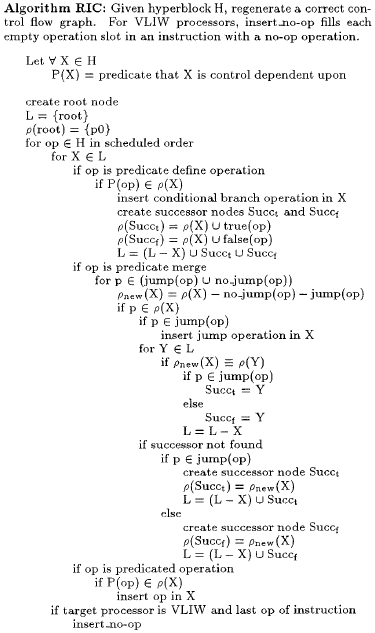
\includegraphics[width=0.9\linewidth]{mechanism/RIC}